\chapter{Исследовательская часть}

Цель исследования: провести уменьшение вектора файла методом главных компонент.

\section{Оборудование}

Характеритстики ноутбука:
\begin{itemize}
	\item процессор intel-core i5-12500H
	\item озу 16 Гб DDR4
	\item ос Windows 11 \cite{lib:windows}
\end{itemize}

\section{Степень различия до и после РСА}\label{diff}

Для выяснения степени различия между двумя матрицами используется косинусная мера близости, 
в которую передается предварительно преобразованная в одномерный вектор матрица близости.
Числа в таблице получаются при сравнении матриц до и после РСА.

\begin{table}[H]
    \centering
    \begin{tabular}{|l|c|c|}
    \hline
    \textbf{Метрика}                                   & \textbf{Обычные вектора} & \textbf{Нормализированные вектора} \\ \hline
    Косинусная мера близости                          & 0.1746                   & 0.2269                             \\ \hline
    Корреляция Пирсона                                & 0.1780                   & 0.2363                             \\ \hline
    Жаккард                                           & 0.8032                   & 0.7783                             \\ \hline
    \end{tabular}
    \caption{Сравнение степеней различия для обычных и нормализированных векторов}
    \label{tab:similarity}
\end{table}
    
\section{Графики}

\begin{figure}[H]
    \begin{minipage}[H]{0.5\linewidth}
        \center{\includegraphics[width=1.2\linewidth]{C:/MGTU/baseAI/lr7/results/HeatmapCos.png}}
        а) До применения РСА
    \end{minipage}
    \begin{minipage}[H]{0.5\linewidth}
        \center{\includegraphics[width=1.2\linewidth]{C:/MGTU/baseAI/lr8_git/bag23u045/report/images/HeatmapCos.png}}
        б) После применения РСА
    \end{minipage}
    \caption{Сравнение косинусной меры близости на обычных векторах до применения РСА и после применения РСА}
    \label{fig:minipageHeatmapCos}
\end{figure}

\begin{figure}[H]
    \begin{minipage}[H]{0.5\linewidth}
        \center{\includegraphics[width=1.2\linewidth]{C:/MGTU/baseAI/lr7/results/HeatmapCosNorm.png}}
        а) До применения РСА
    \end{minipage}
    \begin{minipage}[H]{0.5\linewidth}
        \center{\includegraphics[width=1.2\linewidth]{C:/MGTU/baseAI/lr8_git/bag23u045/report/images/HeatmapCosNorm.png}}
        б) После применения РСА
    \end{minipage}
    \caption{Сравнение косинусной меры близости на нормализированных векторах до применения РСА и после применения РСА}
    \label{fig:minipageHeatmapCosNorm}
\end{figure}

\begin{figure}[H]
    \begin{minipage}[H]{0.5\linewidth}
        \center{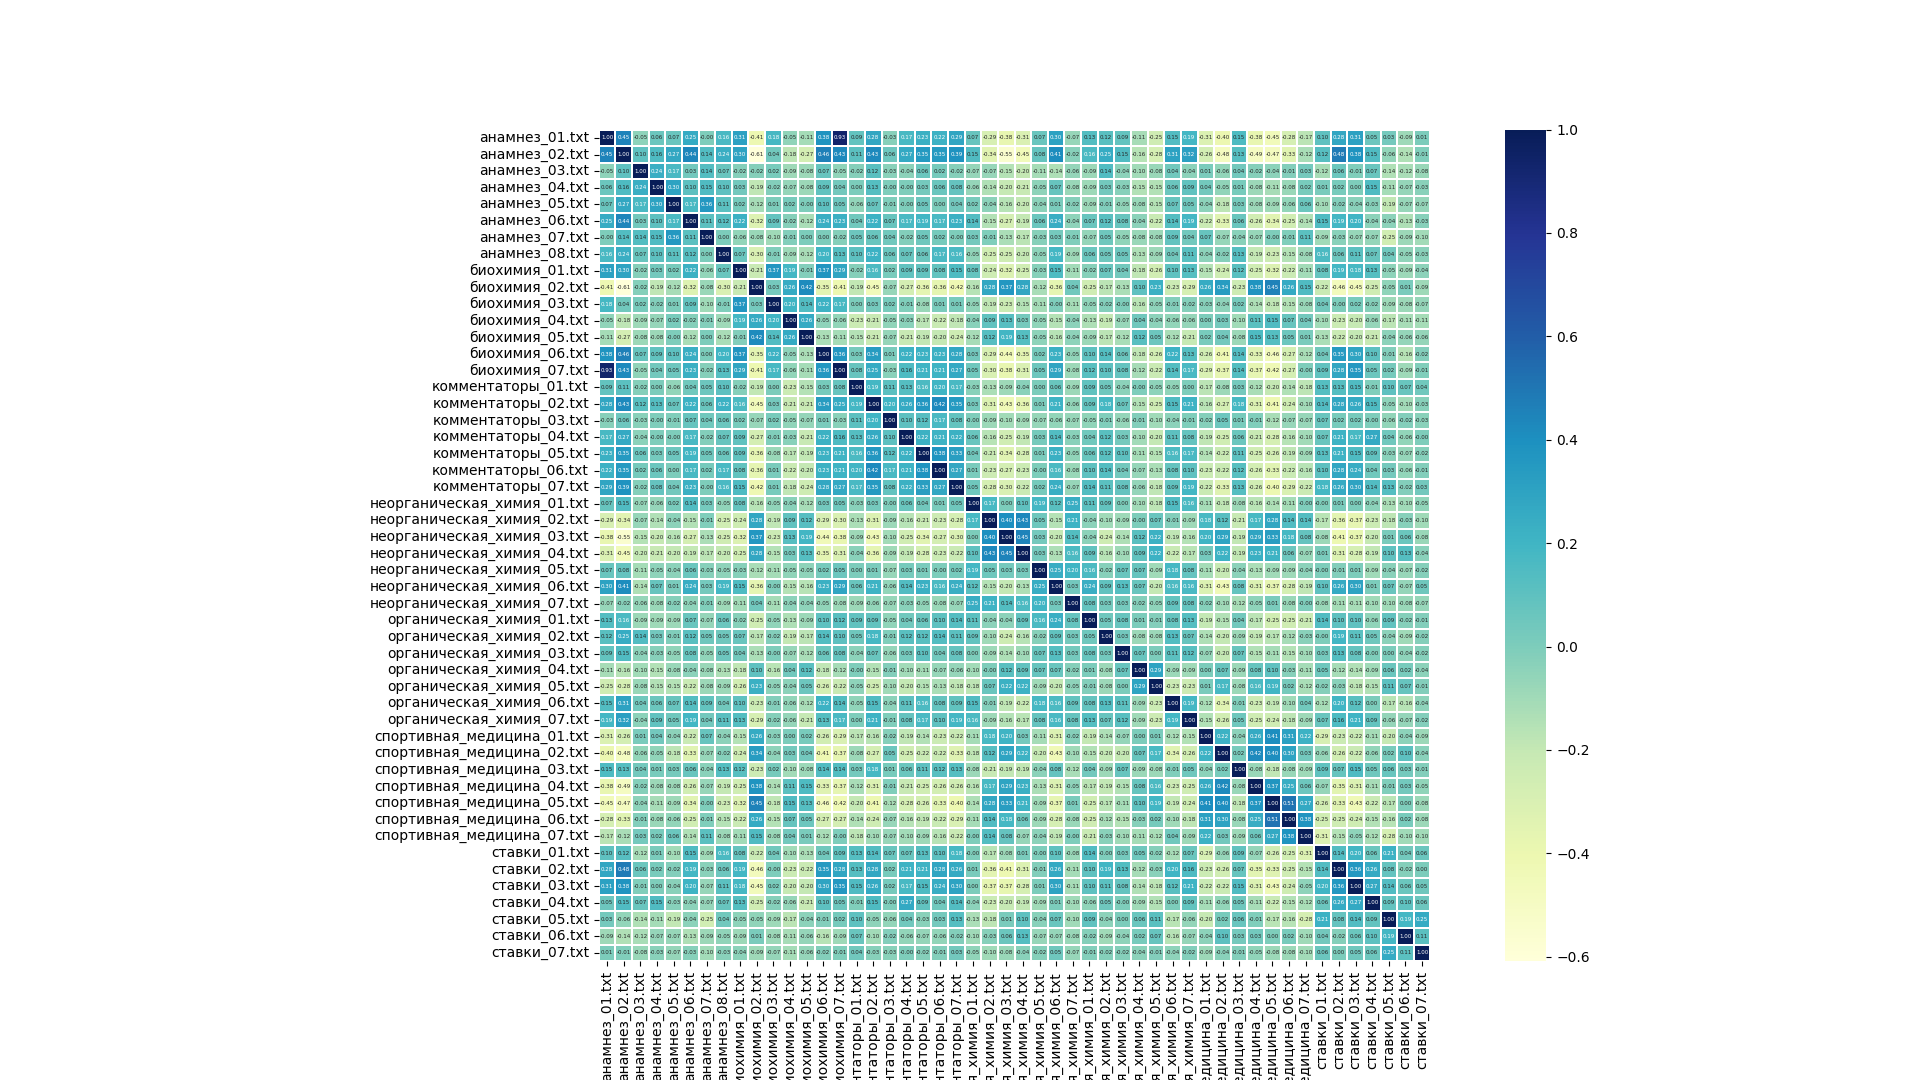
\includegraphics[width=1.2\linewidth]{C:/MGTU/baseAI/lr8_git/bag23u045/report/images/HeatmapPearson.png}}
        а) Тепловая карта, построеная с использование корреляции Пирсона на обычных векторах
    \end{minipage}
    \begin{minipage}[H]{0.5\linewidth}
        \center{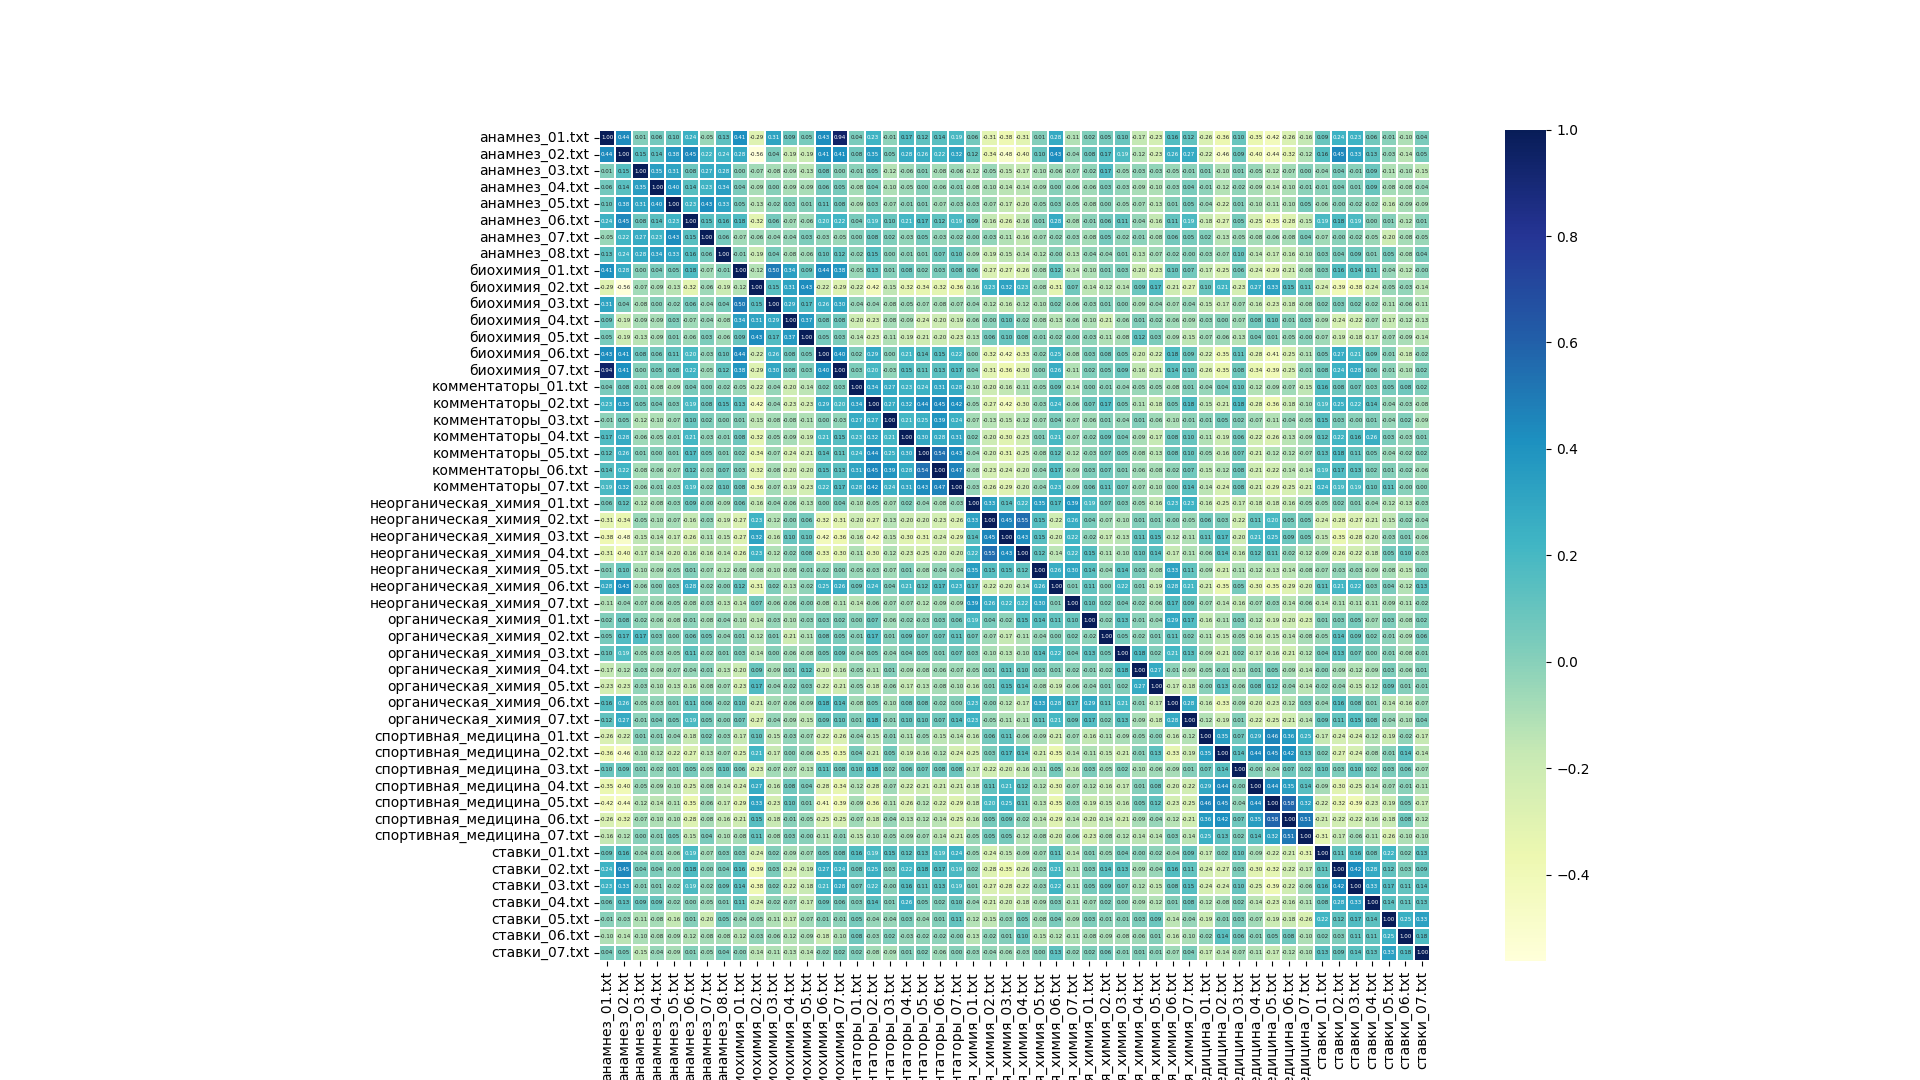
\includegraphics[width=1.2\linewidth]{C:/MGTU/baseAI/lr8_git/bag23u045/report/images/HeatmapPearsonNorm.png}}
        б) Тепловая карта, построеная с использование корреляции Пирсона на нормализированных векторах
    \end{minipage}
    \caption{Сравнение корреляцией Пирсона после применения РСА на обычных векторах и нормализированных векторах}
    \label{fig:minipageHeatmapPearson}
\end{figure}

\begin{figure}[H]
    \begin{minipage}[H]{0.5\linewidth}
        \center{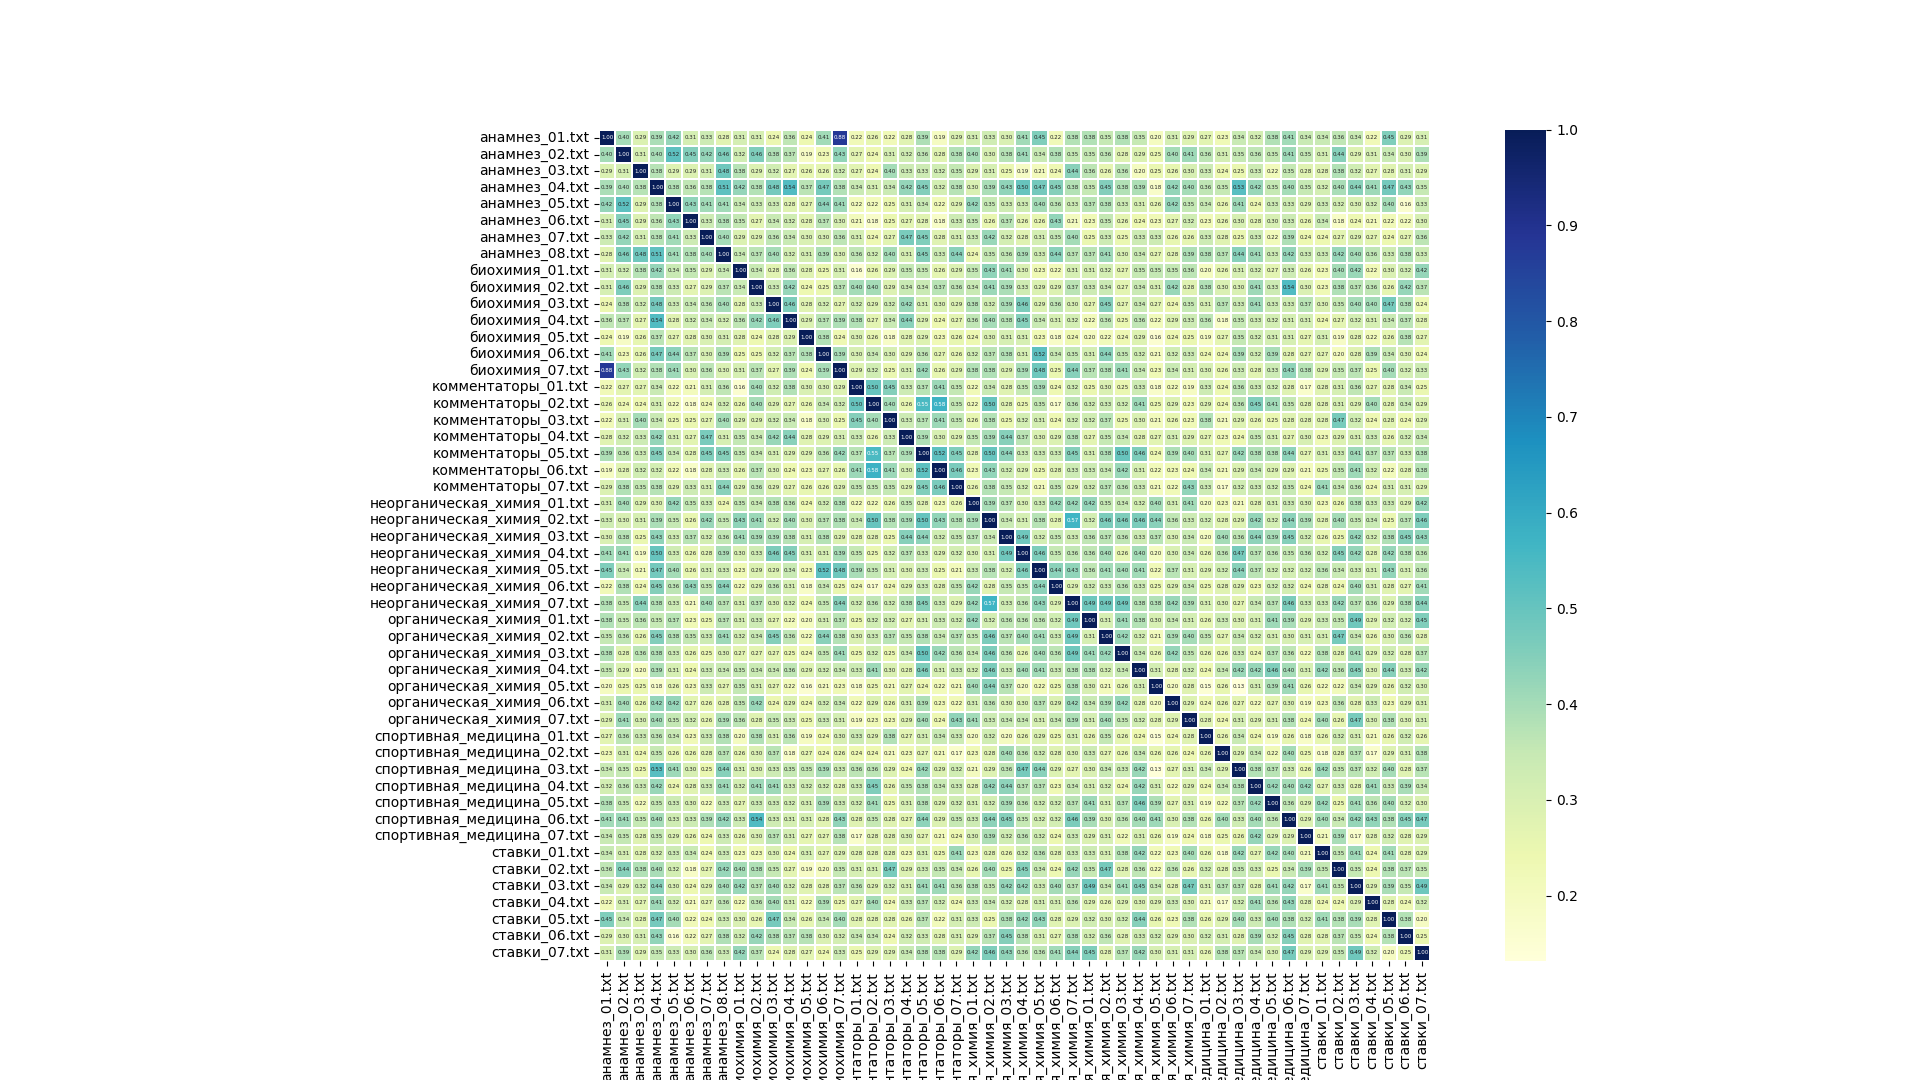
\includegraphics[width=1.2\linewidth]{C:/MGTU/baseAI/lr8_git/bag23u045/report/images/HeatmapJac.png}}
        а) Тепловая карта, построеная с использование корреляции Жаккарда на обычных векторах
    \end{minipage}
    \begin{minipage}[H]{0.5\linewidth}
        \center{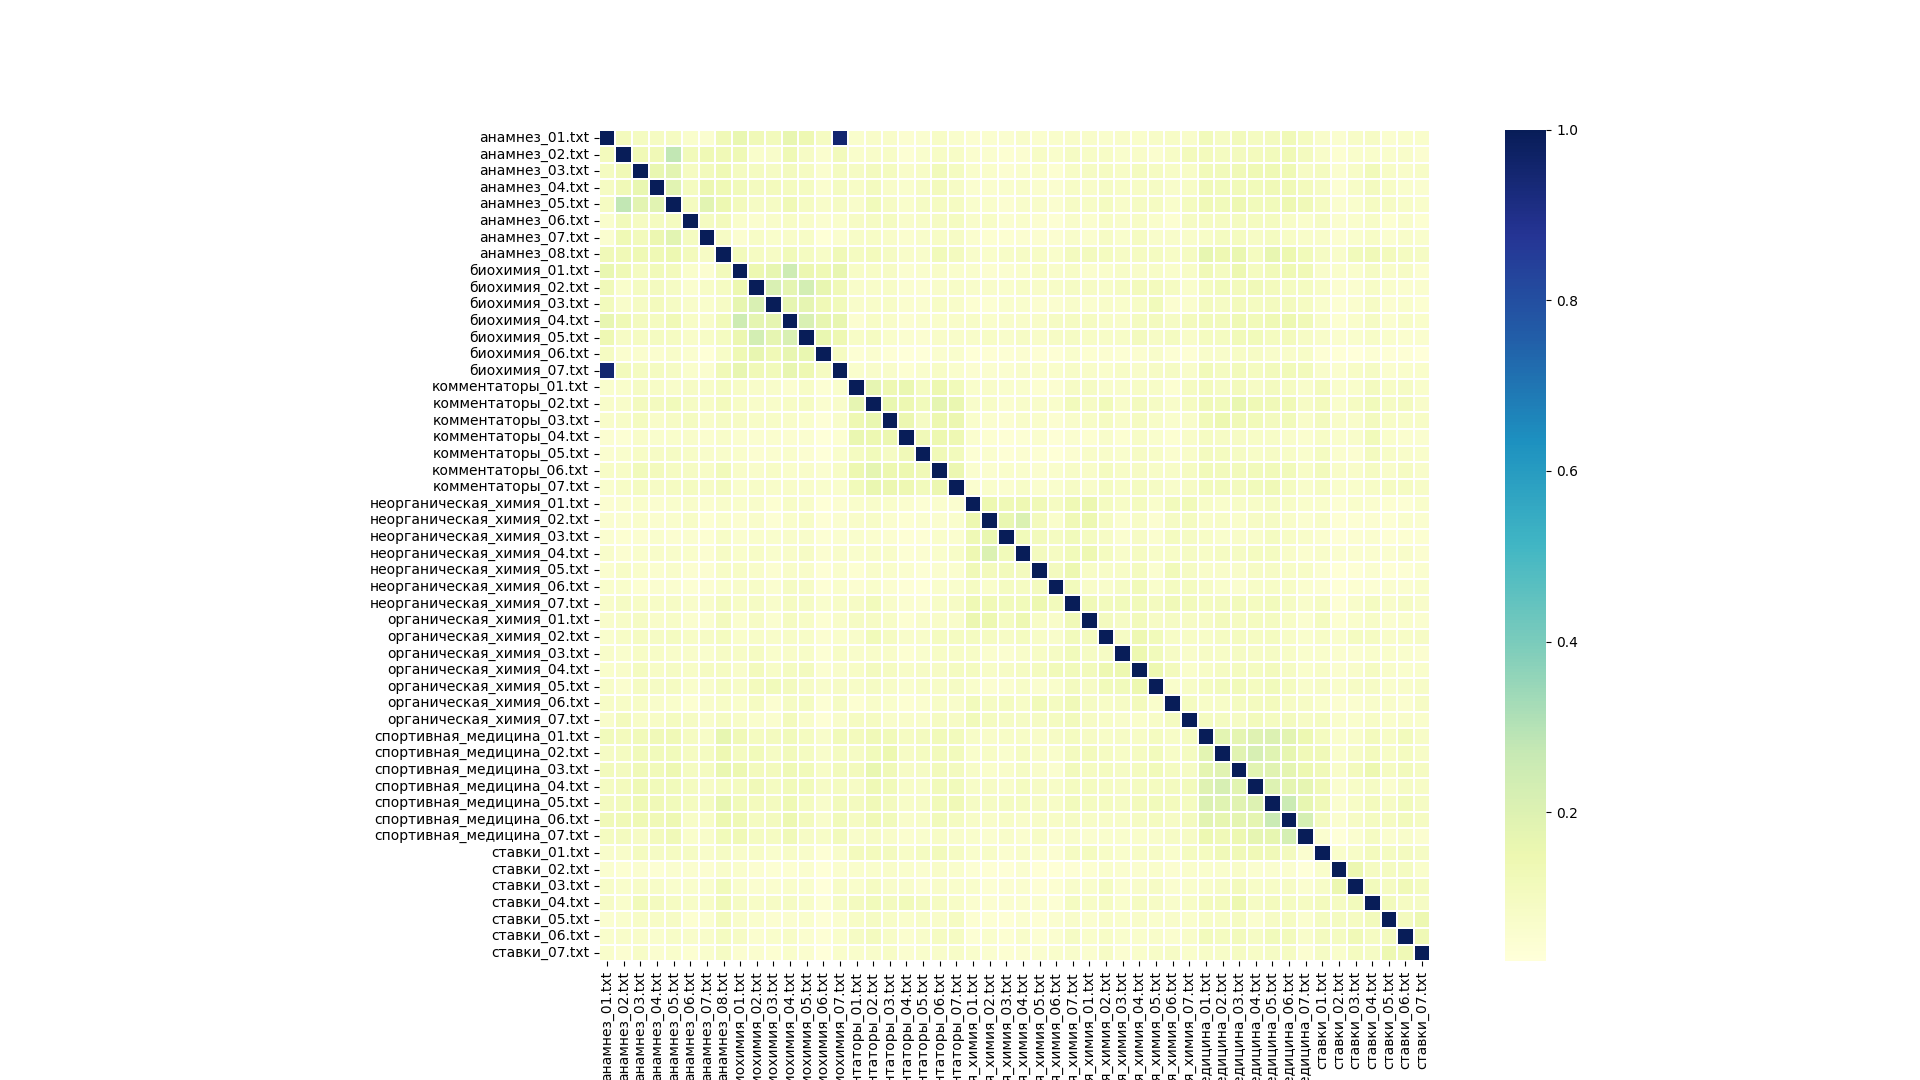
\includegraphics[width=1.2\linewidth]{C:/MGTU/baseAI/lr8_git/bag23u045/report/images/HeatmapJacNorm.png}}
        б) Тепловая карта, построеная с использование корреляции Жаккарда на нормализированных векторах
    \end{minipage}
    \caption{Сравнение метода Жаккарда после применения РСА на обычных векторах и нормализированных векторах}
    \label{fig:minipageHeatmapJac}
\end{figure}

\section{Вывод}

Проведённое уменьшение векторов файлов методом главных компонент изменяет их взаимное отношение, 
что подтверждается изменениями в тепловых картах и числовыми показателями таблицы (см. \ref{diff}). 
Несмотря на уменьшение размерности, исходные структуры векторов сохраняются, 
однако степень схожести после применения метода PCA варьируется в зависимости от типа метрики и нормализации векторов.

\clearpage
